\section{Introduction}
With both original measurements of the phantom and distorted data points, distortion or correction 
parameters can now be calculated 

\begin{eqnarray} \label{eq:spherical_harmonics}
\bar{x_i} = x_i(1 + K_{x_0}(x_i^2 + y_i^2) + K_{x_1}z_i^2 + K_{x_2}z_i^2(x_i^2 + y_i^2) 
+ K_{x_3}(x_i^2 + y_i^2)^2 + K_{x_4}z_i^4) \\
\bar{y_i} = y_i(1 + K_{y_0}(x_i^2 + y_i^2) + K_{y_1}z_i^2 + K_{y_2}z_i^2(x_i^2 + y_i^2) 
+ K_{y_3}(x_i^2 + y_i^2)^2 + K_{y_4}z_i^4) \\
\bar{z_i} = z_i(1 + K_{z_0}(x_i^2 + y_i^2) + K_{z_1}z_i^2 + K_{z_2}z_i^2(x_i^2 + y_i^2) 
+ K_{z_3}(x_i^2 + y_i^2)^2 + K_{z_4}z_i^4)
\end{eqnarray}

where $(\bar{x}_i, \bar{y}_i, \bar{z}_i)$ and $(x_i, y_i, z_i)$ represent distorted and corrected data sets.
If $(\bar{x}_i, \bar{y}_i, \bar{z}_i)$ is distorted data set, $K_{x_i}, K_{y_i}, K_{z_i}$ would be 
distortion parameters, i.e. parameters used to distort original phantom data. If 
$(\bar{x}_i, \bar{y}_i, \bar{z}_i)$ and $(x_i, y_i, z_i)$ are swapped, $K_{x_i}, K_{y_i}, K_{z_i}$ would work as
correction parameters, i.e. parameters used to convert distorted data points into their original position.
In this case, what need to be calculated is correction parameters which will be used to correct the
distortions inside MR images.

Both $(x_i, y_i, z_i)$ and $(\bar{x}_i, \bar{y}_i, \bar{z}_i)$ have to be in DICOM coordinate, i.e. relative
coordinate from gradient isocenter. The gradient isocenter computed in early chapters are using data points
extracted from MR images, so it can be used to convert data points from MR images into DICOM coordinate, but 
not the corrected data. 

\section{XY Axis Distortion Correction Parameters Calculation}
This section describes how to setup and calculate the X and Y axis correction parameters.

Consider using two data points from two separate MR tubes in the same xy plane, two equations could be
setup:

\begin{eqnarray} \label{eq:xy_setup_sample}
\bar{x_0} = x_0(1 + K_{x_0}(x_0^2 + y_0^2) + K_{x_1}z_0^2 + K_{x_2}z_0^2(x_0^2 + y_0^2) 
+ K_{x_3}(x_0^2 + y_0^2)^2 + K_{x_4}z_0^4)  \\
\bar{x_1} = x_1(1 + K_{x_1}(x_1^2 + y_1^2) + K_{x_1}z_1^2 + K_{x_2}z_1^2(x_1^2 + y_1^2) 
+ K_{x_3}(x_1^2 + y_1^2)^2 + K_{x_4}z_1^4) 
\end{eqnarray}

where $(x_0, y_0, z_0)$ and $(x_1, y_1, z_1)$ are DICOM coordinates of the two points from distorted space, 
which are known, and $(\bar{x}_0, \bar{y}_0, \bar{z}_0)$, $(\bar{x}_1, \bar{y}_1, \bar{z}_1)$ are DICOM 
coordinates of two points from corrected spaces which are unknown. However, the exact distance of tube
spacings are known, as well as the distance between opposite side of tubes. So 
$(\delta{x}_{0,1}, \delta{y}_{0,1}, \delta{z}_{0,1})$ can be calculated using 

\begin{equation}
  (\delta{x}_{i,j}, \delta{y}_{i,j}, \delta{z}_{i,j}) = 
  (\bar{x}_i, \bar{y}_i, \bar{z}_i) - (\bar{x}_j, \bar{y}_j, \bar{z}_j)
\end{equation}

where $i, j$ should belong to the same row of tubes for calculating X-axis correction parameters 
or should belong to the same column of tubes for calculating Y-axis correction parameters. 
figure \ref{fig:correction_tube_pairing_xy} shows how the pairing is done for x, and y axis. 

\begin{figure}[htb]
  \begin{minipage}[b]{2.75in}
    \centering
    \centerline{\mbox{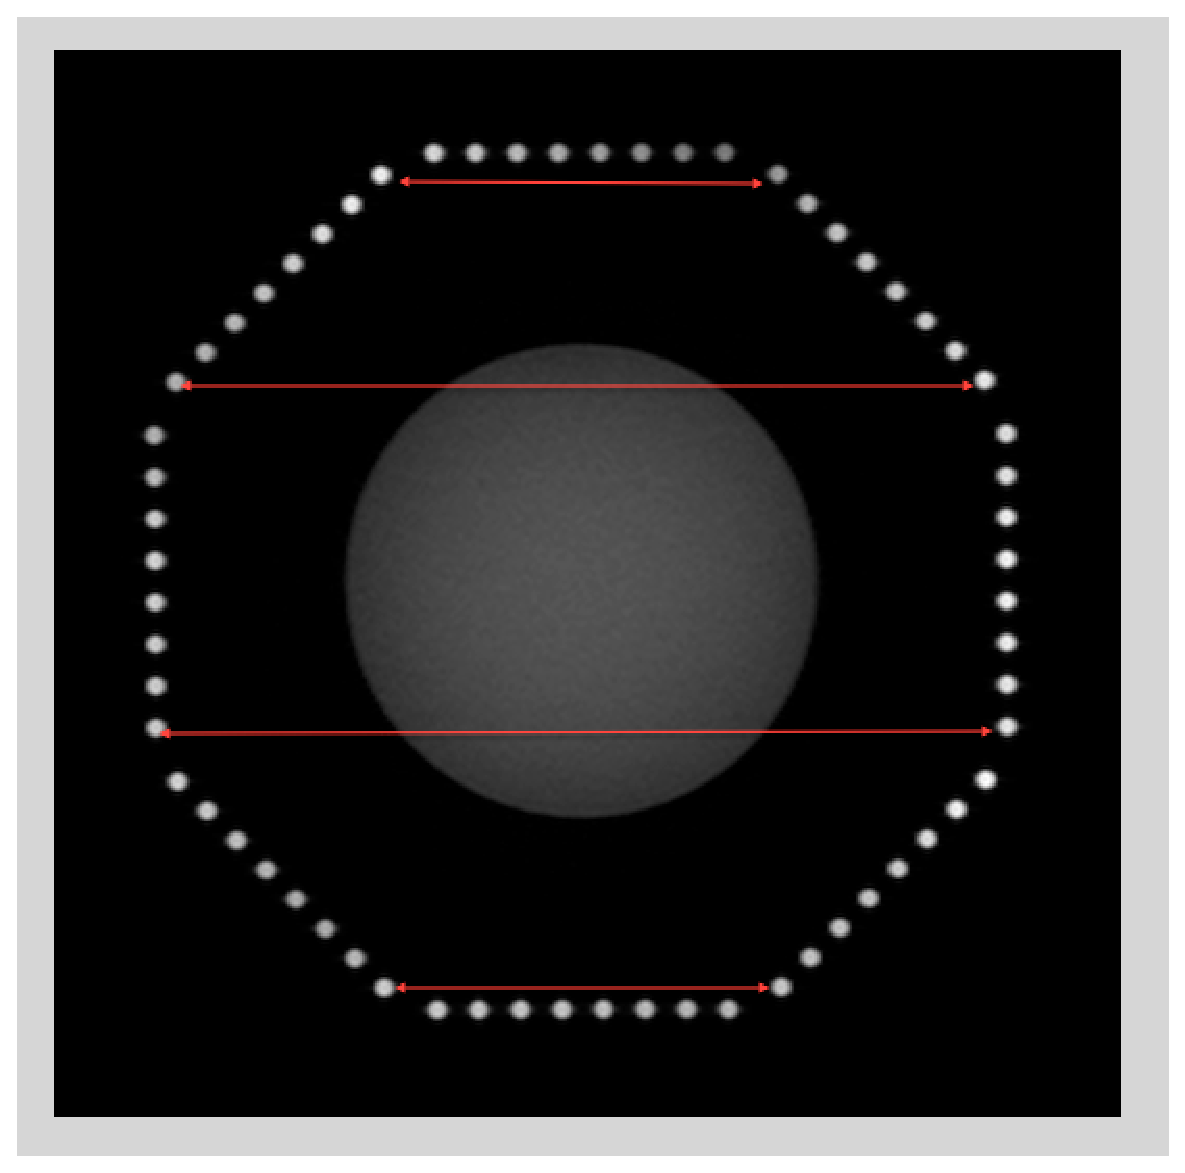
\includegraphics[width=2.75in]{parameters/images/tubes_pairing_x.eps}}}
    \centerline{\emph{(a)}}
  \end{minipage}
  \begin{minipage}[b]{2.75in}
    \centering
    \centerline{\mbox{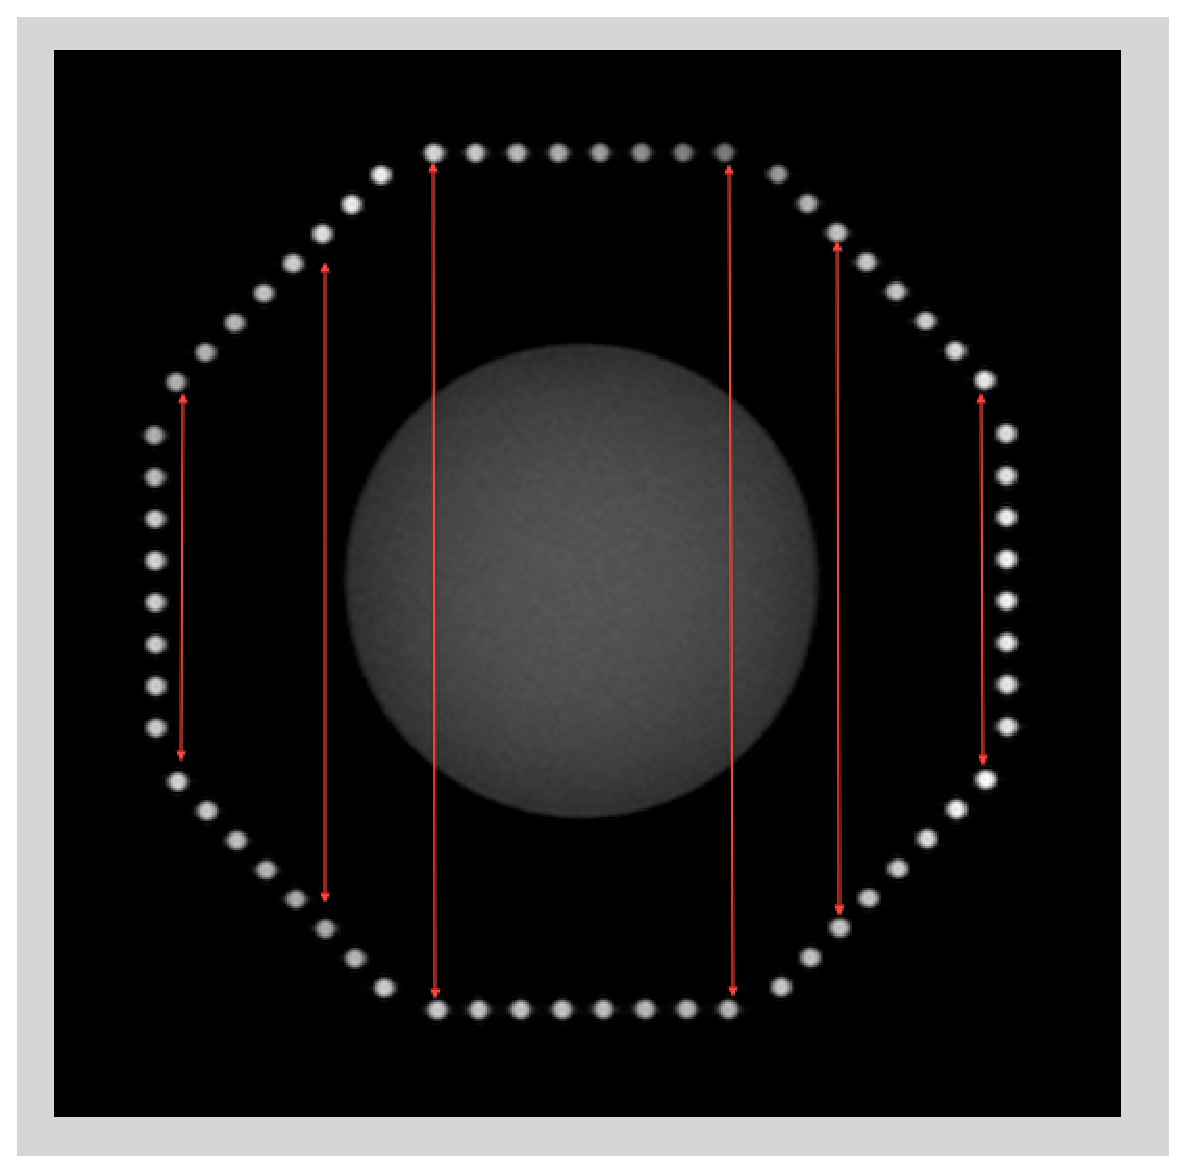
\includegraphics[width=2.75in]{parameters/images/tubes_pairing_y.eps}}}
    \centerline{\emph{(b)}}
  \end{minipage}
  \caption{\emph{Pairing of MR tubes. (a) Pairing for X-axis (b) Pairing for Y-axis}}
  \label{fig:correction_tube_pairing_xy}
\end{figure}

For each pairing, a new formula is produced.
\begin{eqnarray} 
  \delta{\bar{x_{ij}}} & = & \delta{x_{ij}}(1 + K_{x_0}((x_i^2 + y_i^2) - (x_j^2 + y_j^2)) + \nonumber\\
  & & K_{x_1}(z_i^2 - z_j^2) + \nonumber\\
  & & K_{x_2}(z_i^2(x_i^2 + y_i^2)- z_j^2(x_j^2 + y_j^2)) + \nonumber\\
  & & K_{x_3}((x_i^2 + y_i^2)^2 - (x_j^2 + y_j^2)^2) + \nonumber\\
  & & K_{x_4}(z_0^4 - z_j^4)) \\
  \delta{\bar{y_{ij}}} & = & \delta{y_{ij}}(1 + K_{y_0}((x_i^2 + y_i^2) - (x_j^2 + y_j^2)) + \nonumber\\
  & & K_{y_1}(z_i^2 - z_j^2) + \nonumber\\
  & & K_{y_2}(z_i^2(x_i^2 + y_i^2)- z_j^2(x_j^2 + y_j^2)) + \nonumber\\
  & & K_{y_3}((x_i^2 + y_i^2)^2 - (x_j^2 + y_j^2)^2) + \nonumber\\
  & & K_{y_4}(z_0^4 - z_j^4))
\end{eqnarray}

\section{Z Axis Distortion Correction Parameters Calculation}

Similarly to xy correction, we pair up surfaces of water tanks. Figure \ref{fig:correction_surface_pairing}, 
show the pairing.

\begin{figure}[htb]
  \begin{minipage}[b]{0.8\linewidth}
    \centering
    \centerline{\mbox{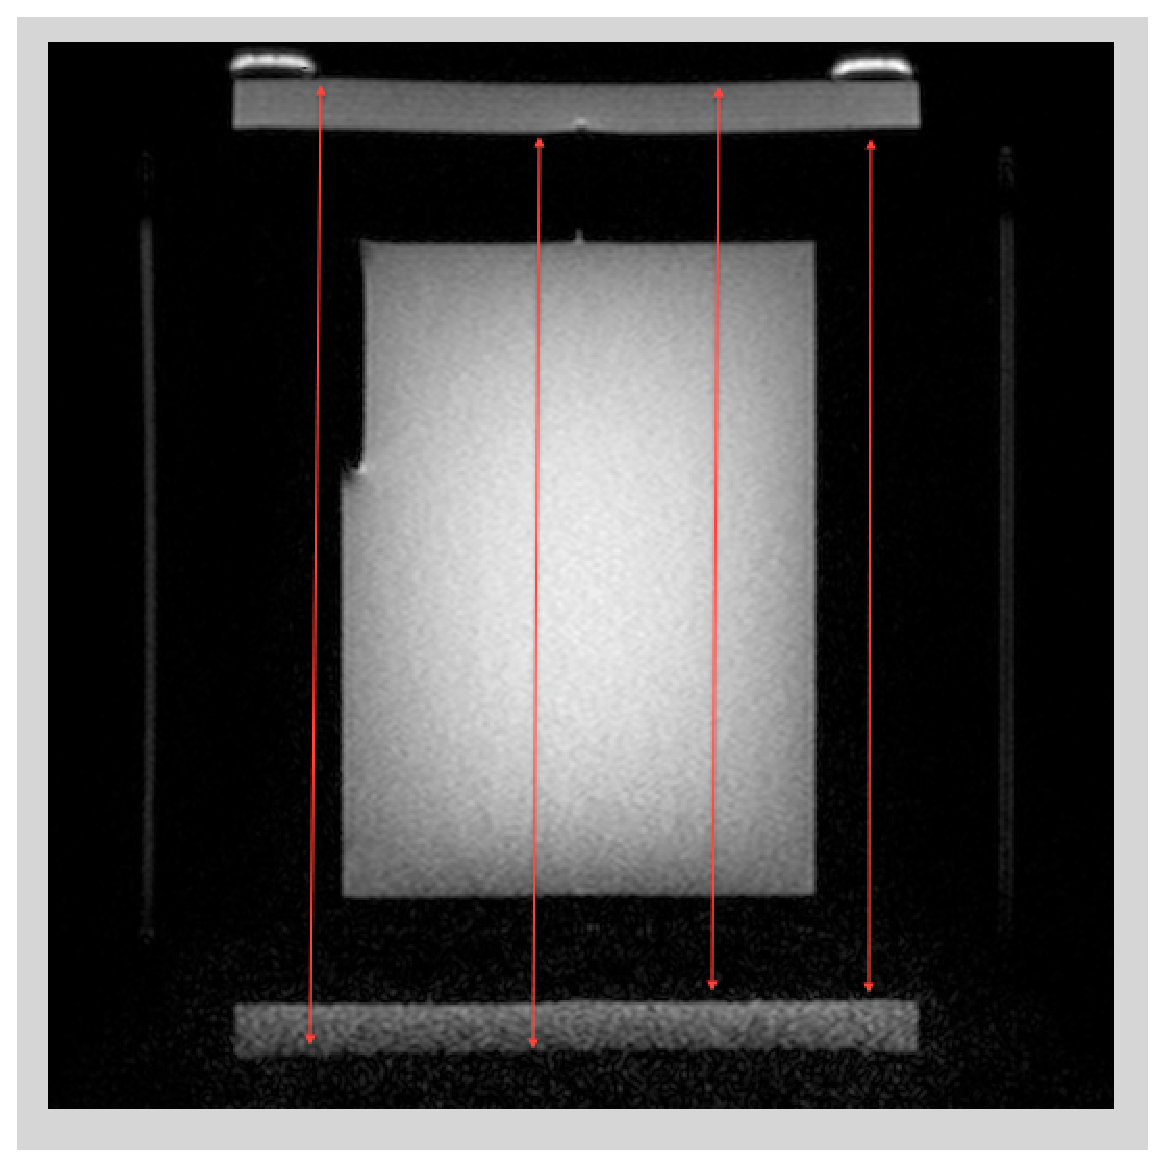
\includegraphics[width=0.8\linewidth]{parameters/images/surface_pairing_z.eps}}}
    % \centerline{\emph{(a)}}
  \end{minipage}
  \caption{\emph{Pairing of tank surfaces. }}
  \label{fig:correction_surface_pairing}
\end{figure}

And the formula we used for z axis correction is:
\begin{eqnarray}
  \delta{\bar{z_{ij}}} & = & \delta{z_{ij}}(1 + K_{z_0}((x_i^2 + y_i^2) - (x_j^2 + y_j^2)) + \nonumber\\
  & & K_{z_1}(z_i^2 - z_j^2) + \nonumber\\
  & & K_{z_2}(z_i^2(x_i^2 + y_i^2)- z_j^2(x_j^2 + y_j^2)) + \nonumber\\
  & & K_{z_3}((x_i^2 + y_i^2)^2 - (x_j^2 + y_j^2)^2) + \nonumber\\
  & & K_{z_4}(z_0^4 - z_j^4))  
\end{eqnarray}

% \subsubsection{Accuracy}

% The accuracy has been tested in matlab simulation. XY axis correction tends to stay around within 0.001 mm
% while Y axis correction is around 0.1mm accuracy.

